%----------------------------------------------------------------------------------------
%	PACKAGES AND OTHER DOCUMENT CONFIGURATIONS
%----------------------------------------------------------------------------------------

\documentclass[paper=a4, fontsize=11pt]{scrartcl} % A4 paper and 11pt font size

% ---- Entrada y salida de texto -----

\usepackage[T1]{fontenc} % Use 8-bit encoding that has 256 glyphs
\usepackage[utf8]{inputenc}
%\usepackage{fourier} % Use the Adobe Utopia font for the document - comment this line to return to the LaTeX default

% ---- Idioma --------

\usepackage[spanish, es-tabla]{babel} % Selecciona el español para palabras introducidas automáticamente, p.ej. "septiembre" en la fecha y especifica que se use la palabra Tabla en vez de Cuadro

% ---- Otros paquetes ----
\usepackage{csquotes} %Para permitir el uso de comillas Quotes https://tex.stackexchange.com/questions/36812/isnt-there-any-other-way-of-doing-double-quotes-in-latex-besides
\usepackage[hyphens]{url} % ,href} %para incluir URLs e hipervínculos dentro del texto (aunque hay que instalar href)
\usepackage{hyperref}
\usepackage{color}
\usepackage{graphics,graphicx, floatrow} %para incluir imágenes y notas en las imágenes
\usepackage{graphics,graphicx, float} %para incluir imágenes y colocarlas

\graphicspath {{./img/}}

\usepackage{listings}  %para introducir comandos

\lstdefinestyle{mybash}
{basicstyle=\ttfamily,
  showstringspaces=false,
  commentstyle=\color{red},
  keywordstyle=\color{blue},
  language=bash,
  alsoletter=/,
  basicstyle=\footnotesize,
  numbers=left,
  stepnumber=1,
  showstringspaces=false,
  tabsize=1,
  breaklines=true,
  breakatwhitespace=false,
}
\lstdefinestyle{mysql}
{basicstyle=\ttfamily,
  showstringspaces=false,
  commentstyle=\color{red},
  keywordstyle=\color{blue},
  language=sql,
  basicstyle=\footnotesize,
  numbers=left,
  stepnumber=1,
  showstringspaces=false,
  tabsize=1,
  breaklines=true,
  breakatwhitespace=false,
}


% Para hacer tablas comlejas
%\usepackage{multirow}
%\usepackage{threeparttable}

%\usepackage{sectsty} % Allows customizing section commands
%\allsectionsfont{\centering \normalfont\scshape} % Make all sections centered, the default font and small caps

\usepackage{fancyhdr} % Custom headers and footers
\pagestyle{fancyplain} % Makes all pages in the document conform to the custom headers and footers
\fancyhead{} % No page header - if you want one, create it in the same way as the footers below
\fancyfoot[L]{} % Empty left footer
\fancyfoot[C]{} % Empty center footer
\fancyfoot[R]{\thepage} % Page numbering for right footer
\renewcommand{\headrulewidth}{0pt} % Remove header underlines
\renewcommand{\footrulewidth}{0pt} % Remove footer underlines
\setlength{\headheight}{13.6pt} % Customize the height of the header

\setlength\parindent{0pt} % Removes all indentation from paragraphs - comment this line for an assignment with lots of text

\newcommand{\horrule}[1]{\rule{\linewidth}{#1}} % Create horizontal rule command with 1 argument of height


%----------------------------------------------------------------------------------------
%	TÍTULO Y DATOS DEL ALUMNO
%----------------------------------------------------------------------------------------
\graphicspath{ {img/} }

\title{
\normalfont \normalsize

\includegraphics[width=6cm,height=6cm]{logo}\\
\textsc{\textbf{Bootcamp Especialidad GNU/Linux (2023)}} \\ [25pt] % Your university, school and/or department name(s)
\horrule{0.5pt} \\[0.4cm] % Thin top horizontal rule
\huge Lab 01 - Instalación de una distribución de GNU/Linux \\ % The assignment title
\horrule{2pt} \\[0.5cm] % Thick bottom horizontal rule
}

%https://es.overleaf.com/learn/latex/Inserting_Images
%Ruta relativa de   imagenes

\author{Pedro Antonio Mayorgas Parejo} % Nombre y apellidos

\date{\normalsize\today} % Incluye la fecha actual

%----------------------------------------------------------------------------------------
% DOCUMENTO
%----------------------------------------------------------------------------------------

\begin{document}

\maketitle % Muestra el Título

\newpage %inserta un salto de página

\tableofcontents % para generar el índice de contenidos

\newpage

%----------------------------------------------------------------------------------------
%	Cuestión 1
%----------------------------------------------------------------------------------------

\section{Configuración de la Máquina Virtual}

Se ha utilizado QEMU/KVM como sistema hypervisor baremetal, ya que el sistema operativo base que se utiliza, es una distribución de GNU/Linux, permitiendo que pueda tener todas ventajas de aceleración casi sin penalizaciones en el rendimiento.
\vspace{5mm}

Para la configuración de la máquina virtual, he realizado una configuración base consistente en los siguientes parámetros:

\begin{itemize}
\item 2 VCPU, donde asignamos un mínimo de 2 CPU para la fluidez y la multitarea real.
\item 4096 MiB de Memoria RAM, que aunque sea demasiado para las tareas que se le van a asignar a dicha máquina virutal, nos asegura margen futuro.
\item Disco Virtual formato QCOW2, de un tamaño de 40 GiB. 
\end{itemize}

Pasos seguidos para el proceso de instalación de la distribución en una Máquina Virtual.

\begin{figure}[H]
	\centering
	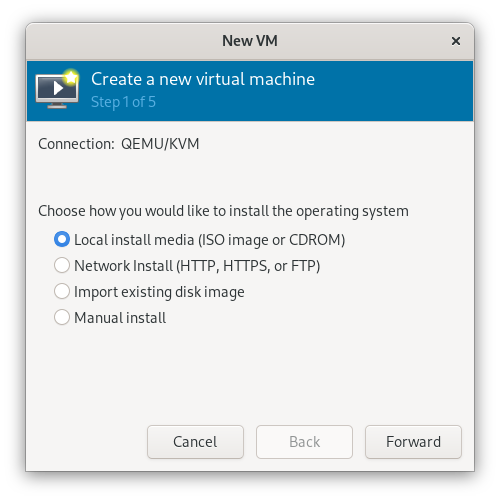
\includegraphics[scale=0.40]{00}
	\caption{La configuración comienza preguntando el medio de instalación.}
\end{figure}

\begin{figure}[H]
	\centering
	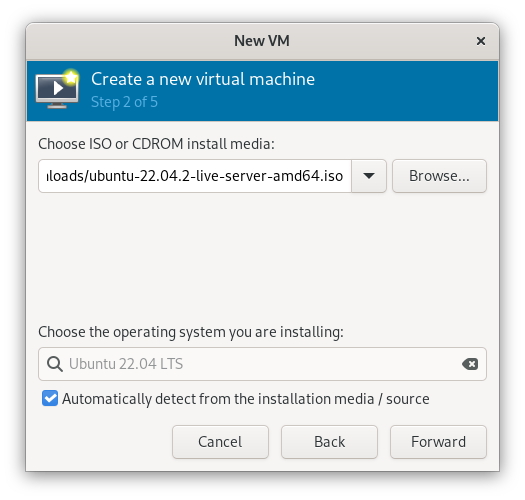
\includegraphics[scale=0.40]{01}
	\caption{Seleccionamos la ISO de Ubuntu Server desde la ruta que queramos y el instalador detecta qué sistema es.}
\end{figure}

\begin{figure}[H]
	\centering
	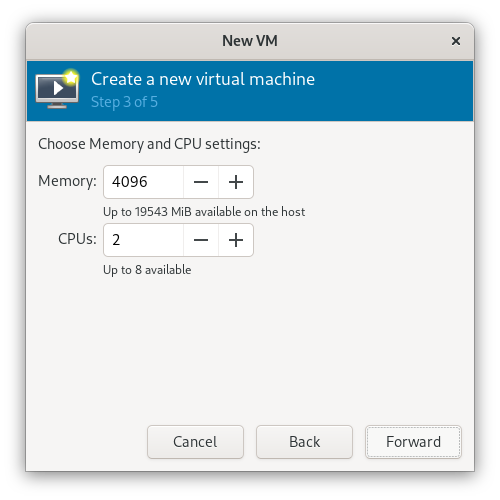
\includegraphics[scale=0.40]{02}
	\caption{Ahora en este punto de la instalación se configura la capacidad de la memoria RAM y CPU.}
\end{figure}

\begin{figure}[H]
	\centering
	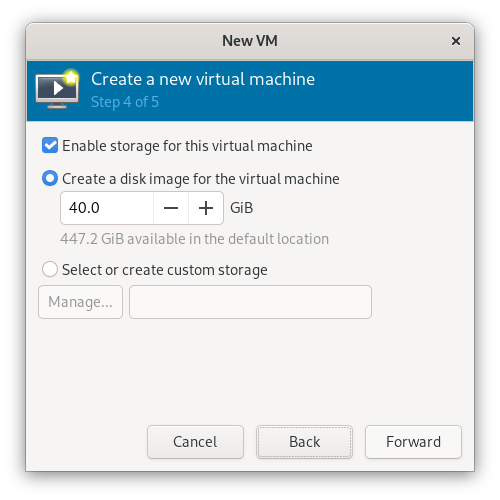
\includegraphics[scale=0.40]{03}
	\caption{Ahora en este punto de la instalación se configura la capacidad de la memoria RAM y CPU.}
\end{figure}

\begin{figure}[H]
	\centering
	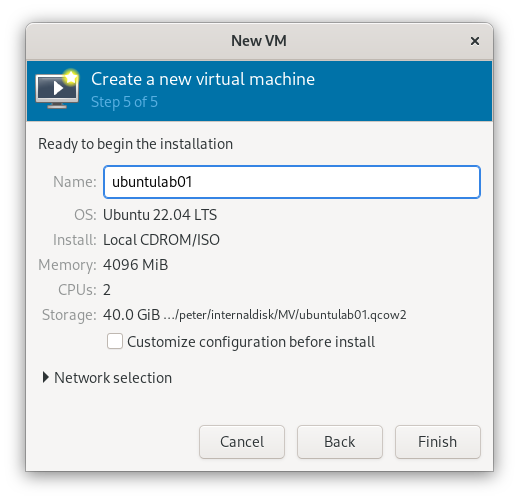
\includegraphics[scale=0.40]{04}
	\caption{Ahora configuramos el disco duro y su capacidad.}
\end{figure}

\begin{figure}[H]
	\centering
	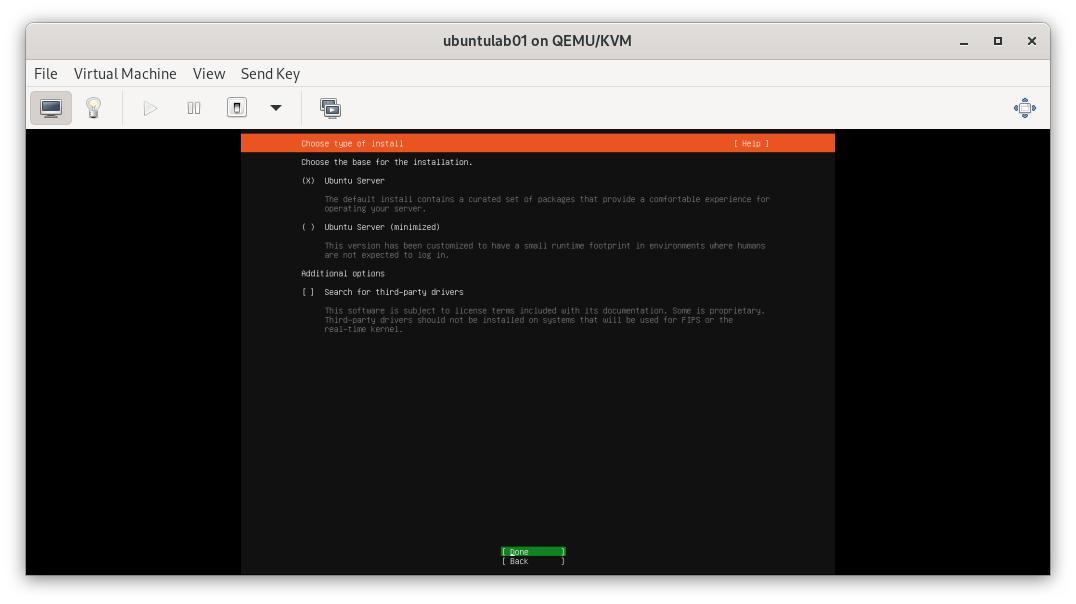
\includegraphics[scale=0.40]{05}
	\caption{Ventana resumen de la máquina.}
\end{figure}

\newpage
\section{Configuración del sistema operativo base}

En la instalación después de seleccionar el idioma y la región, nos mostrará que versión queremos instalar de Ubuntu Server.

\begin{figure}[H]
	\centering
	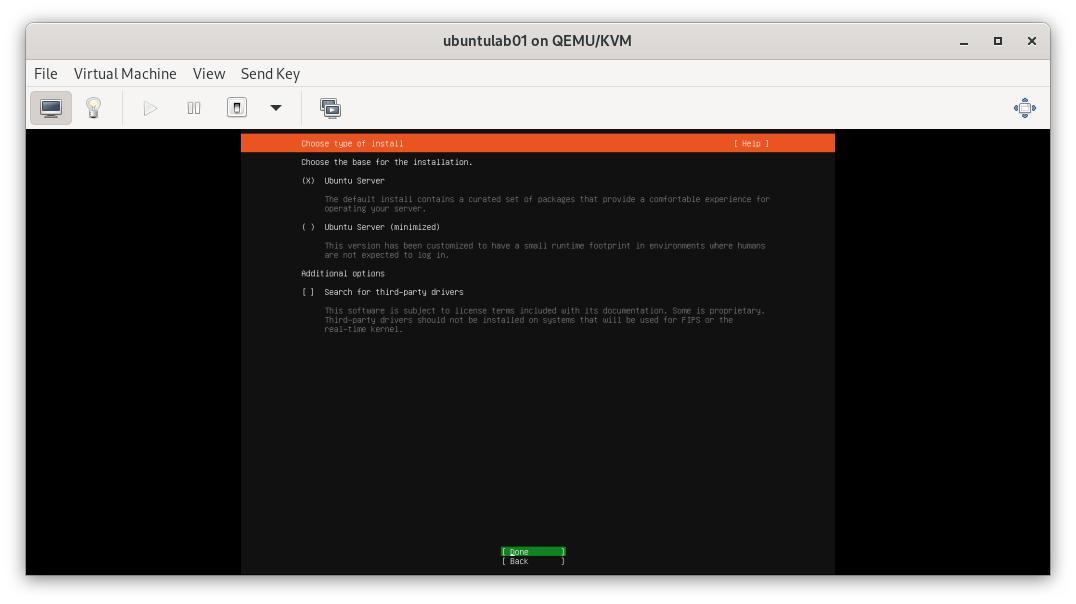
\includegraphics[scale=0.40]{05}
	\caption{Configuración de la versión de Ubuntu Server.}
\end{figure}

Ahora la configuración de la interfaz de red, que es obtenida por DHCPv4 por parte del sistema hypervisor con una puerta de enlace.

\begin{figure}[H]
	\centering
	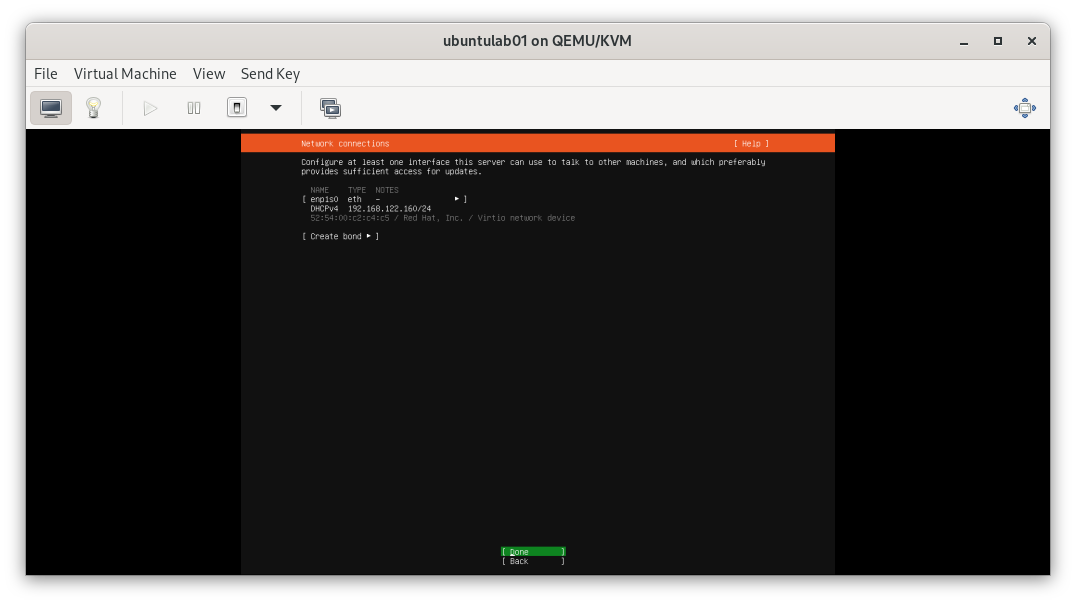
\includegraphics[scale=0.40]{06}
	\caption{Configuración de red.}
\end{figure}

Ahora comenzamos a ver la configuración de los discos, en concreto el particionado. \textbf{Seleccionamos el particionado manual}.

\begin{figure}[H]
	\centering
	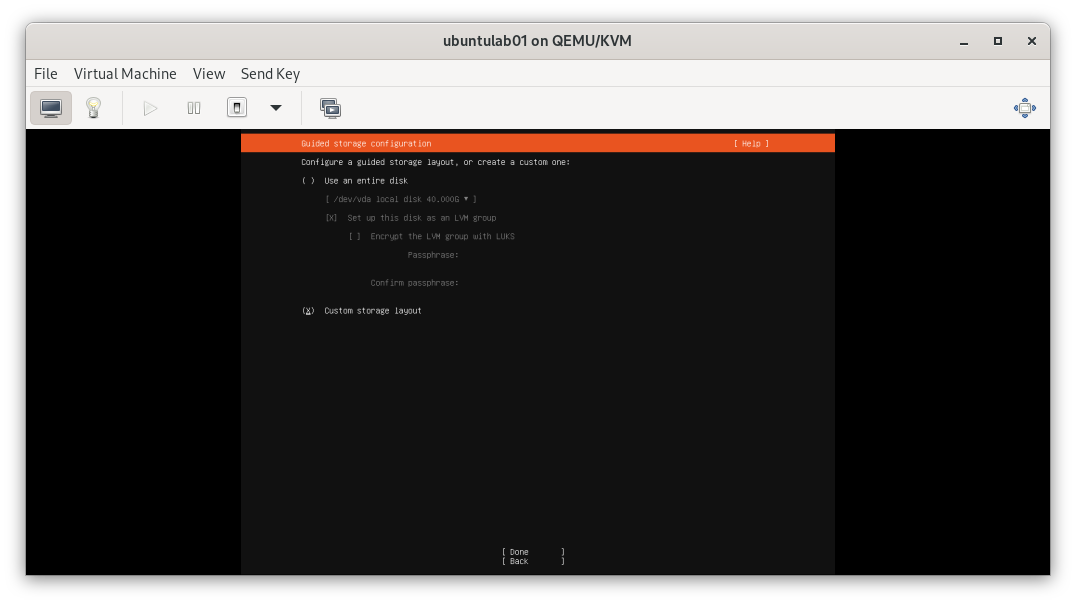
\includegraphics[scale=0.40]{07}
	\caption{Selección del particionado manual.}
\end{figure}

Dentro de la herramienta de particionado manual, debemos crear una partición EFI ESP, que nos permita alojar ahí las configuraciones, variables y ficheros de bootloader (arranque). Dicha partición está formateada en \textbf{fat32}. La partición se monta en \textbf{/boot/efi}.

\begin{figure}[H]
	\centering
	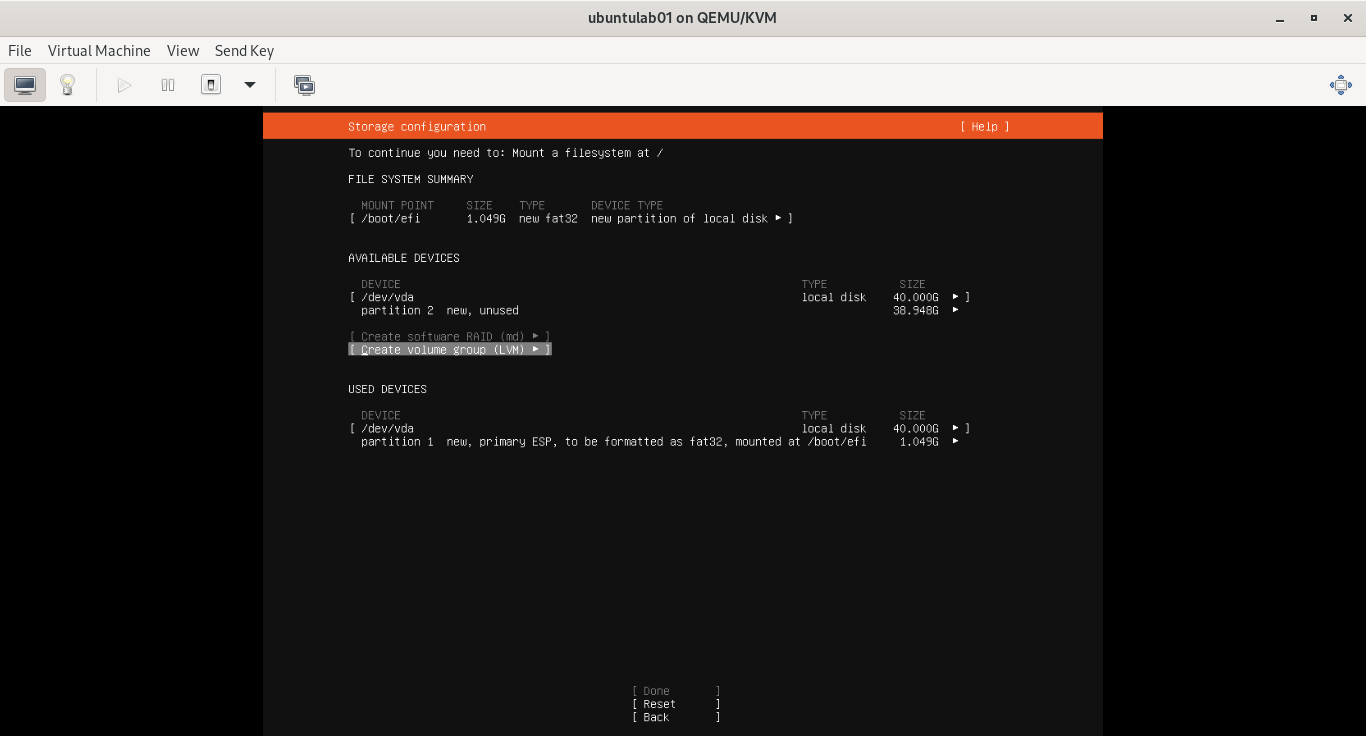
\includegraphics[scale=0.30]{08}
	\caption{Creación de la partición de arranque.}
\end{figure}

Ahora creamos un VG (Volume Group) de LVM a partir de la partición 2 como PV (Physical Volume), donde a partir de dicho VG, se crea un LV (Logical Volume), que funcionará como "partición" que alojará el sistema de ficheros. 

\begin{figure}[H]
	\centering
	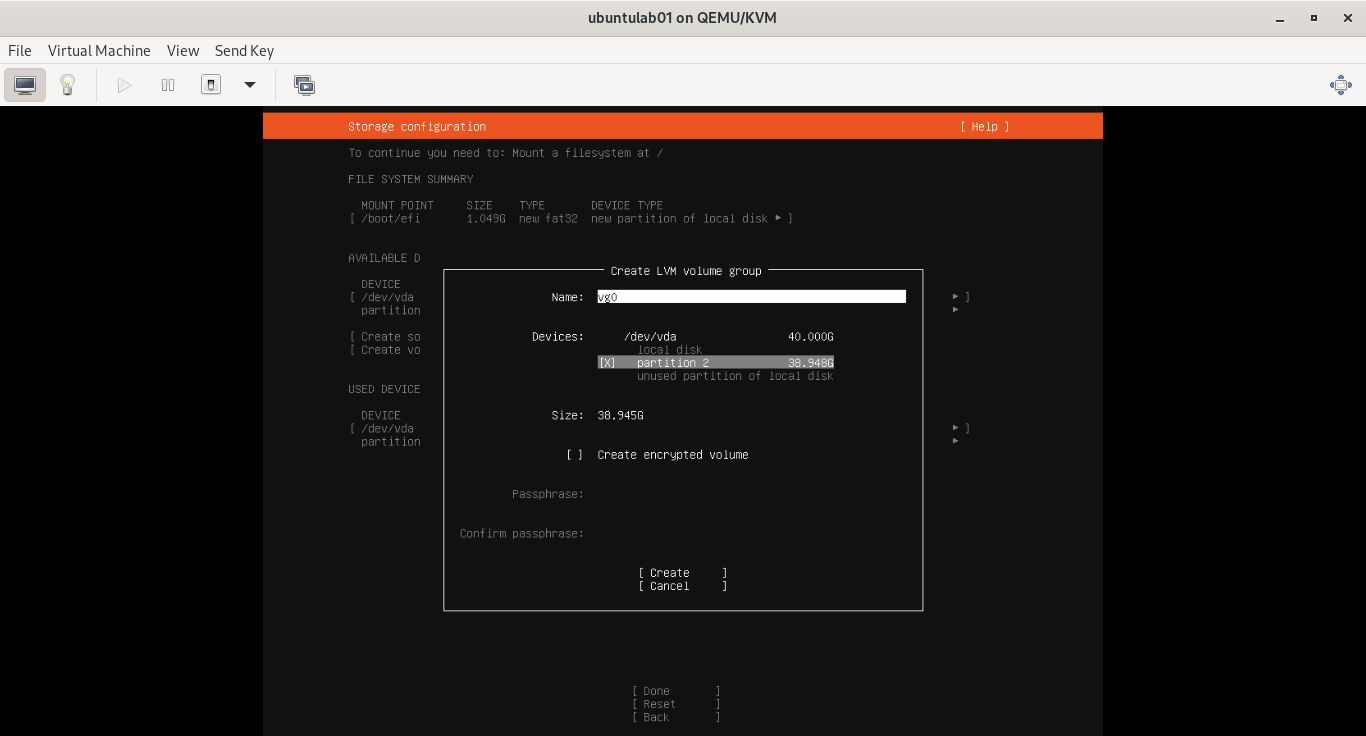
\includegraphics[scale=0.30]{09}
	\caption{Creación del VG a partir del PV de la partición 2.}
\end{figure}

Ahora a continuación, como se ha dicho en el párrafo anterior, tenemos que crear el LV. Para ello nos vamos a \textbf{FREE SPACE} y nos aparecerá la ventana de creación de un LV.

\begin{figure}[H]
	\centering
	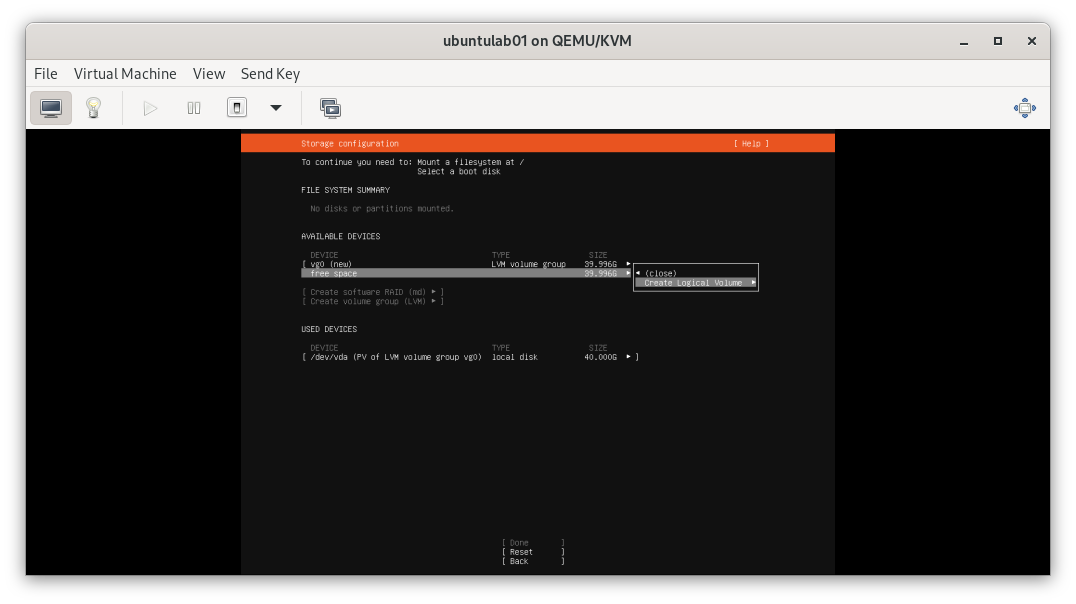
\includegraphics[scale=0.40]{10}
	\caption{Creación del LV menú contextual.}
\end{figure}

Configuración para la raíz \textbf{(ROOT o /)}.

\begin{figure}[H]
	\centering
	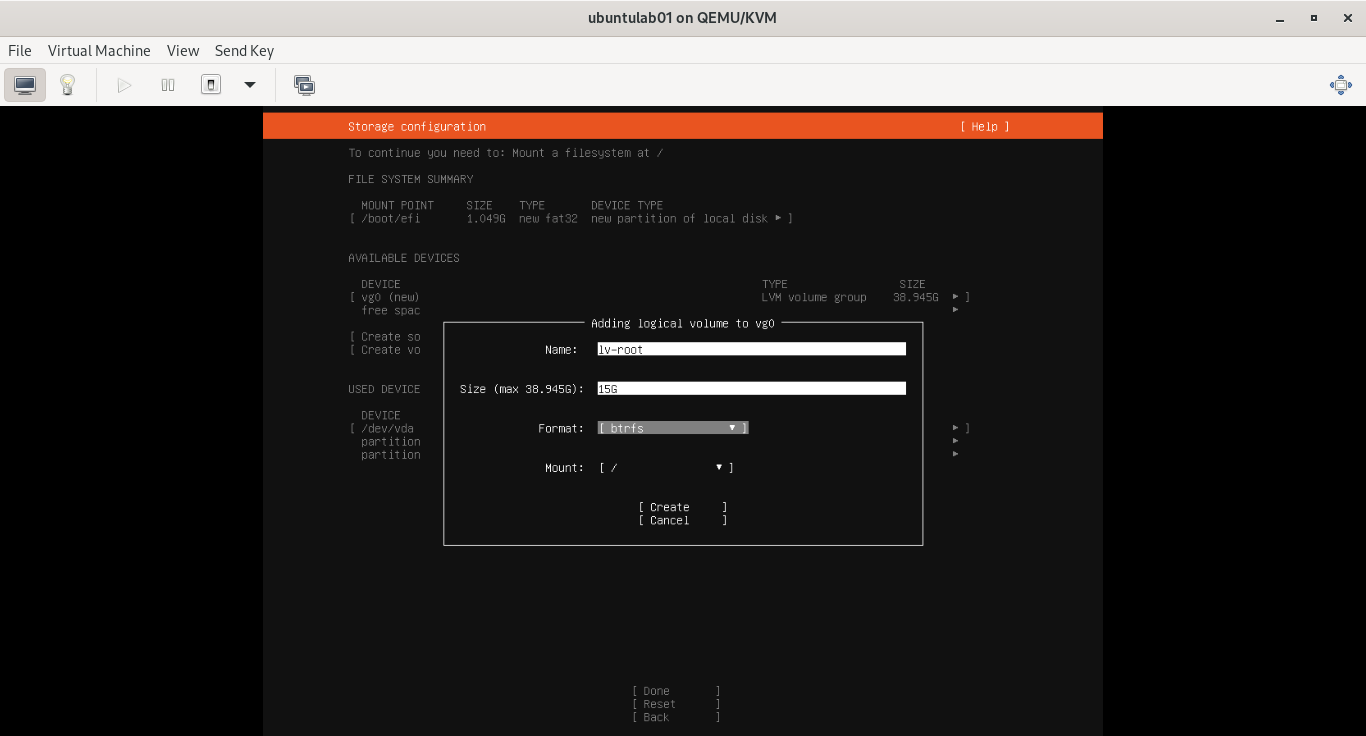
\includegraphics[scale=0.30]{11}
	\caption{Creación del LV de la raíz.}
\end{figure}

Configuración para \textbf{/var.}

\begin{figure}[H]
	\centering
	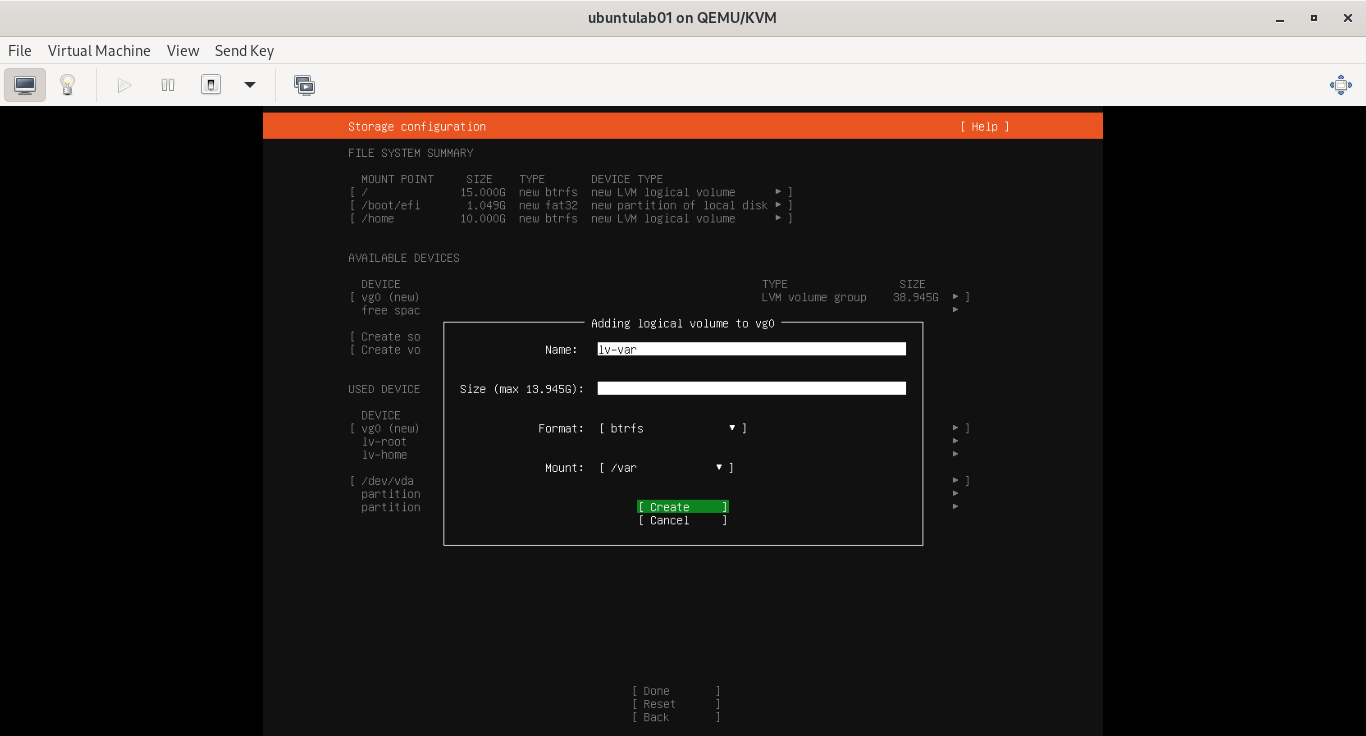
\includegraphics[scale=0.30]{12}
	\caption{Creación del LV de la var.}
\end{figure}

Repetimos los mismos pasos para \textbf{/home} y esta sería la ventana resumen.

\begin{figure}[H]
	\centering
	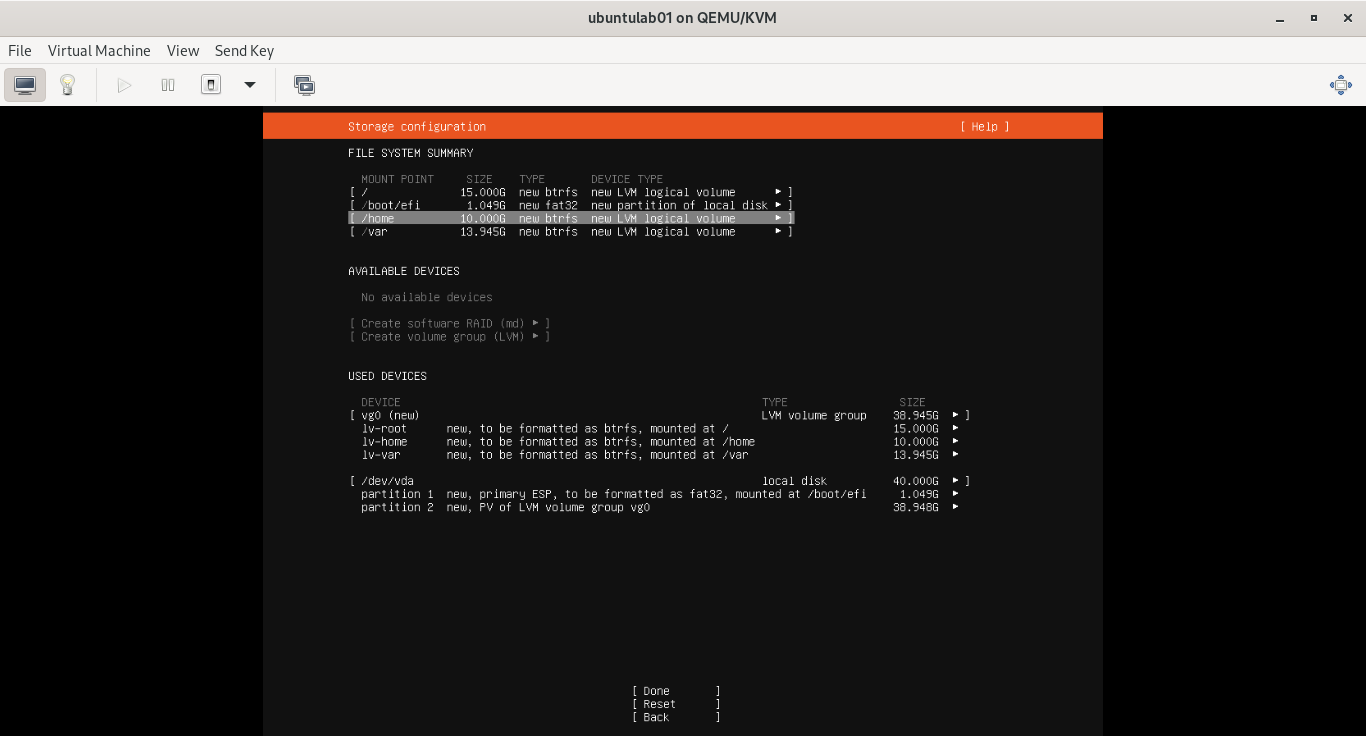
\includegraphics[scale=0.30]{13}
	\caption{Creación del LV de home.}
\end{figure}

Confirmamos el particionado.

\begin{figure}[H]
	\centering
	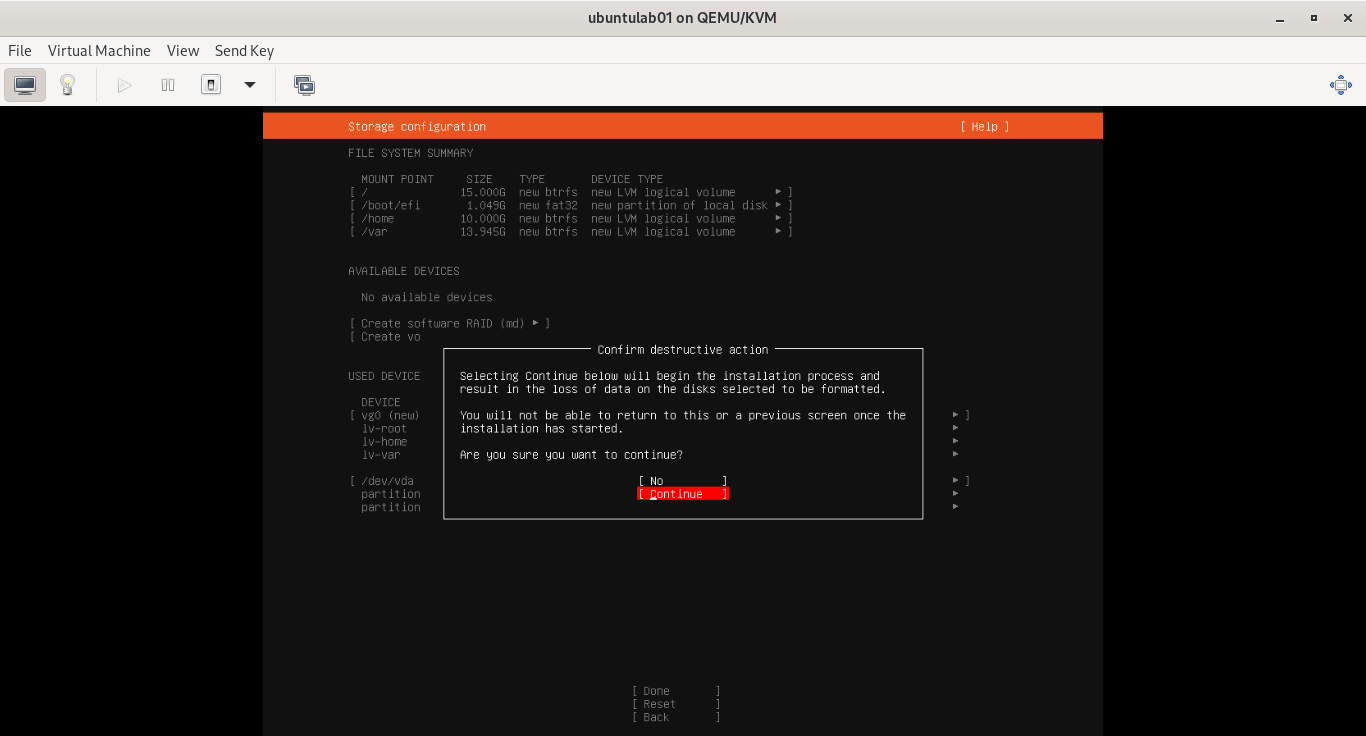
\includegraphics[scale=0.30]{14}
	\caption{Confirmación del particionado.}
\end{figure}

Ahora configuramos el usuario-sudo y la contraseña.

\begin{figure}[H]
	\centering
	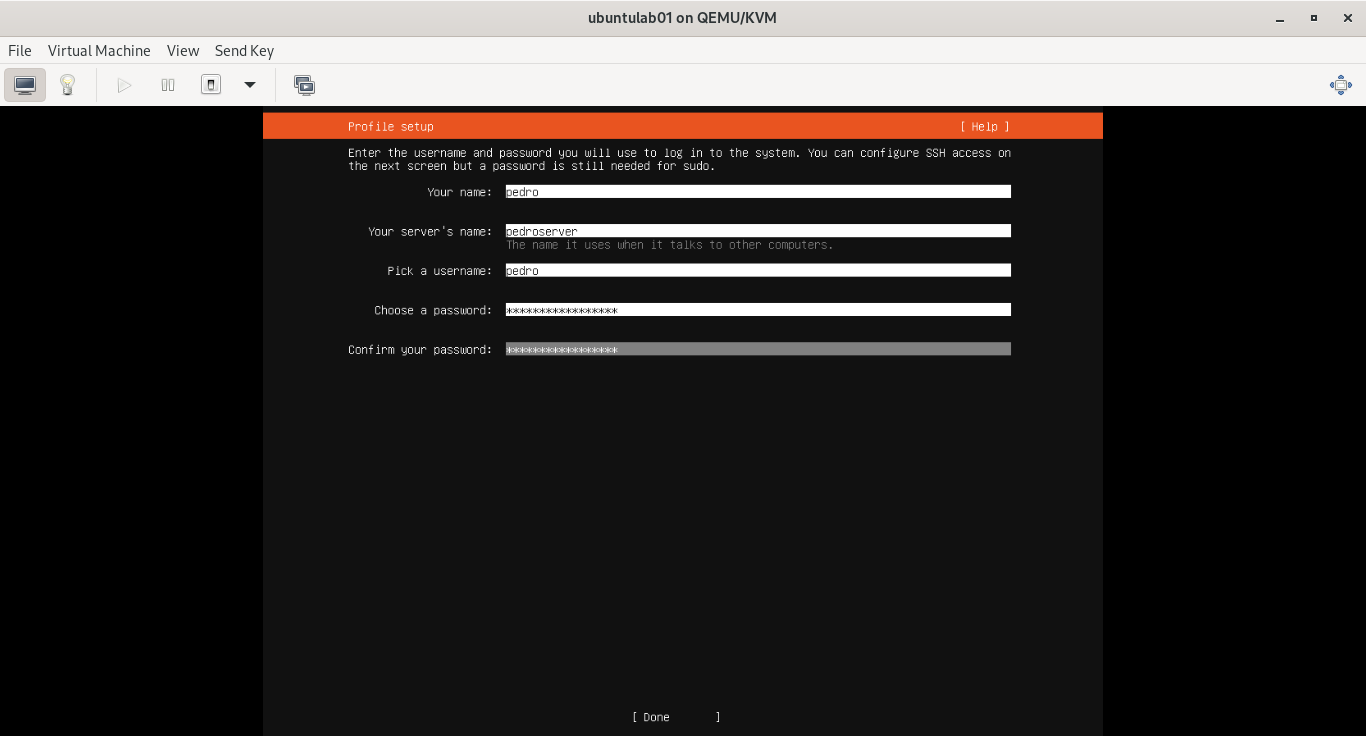
\includegraphics[scale=0.30]{15}
	\caption{Configuración del usuario.}
\end{figure}

Proceso de instalación del sistema base.

\begin{figure}[H]
	\centering
	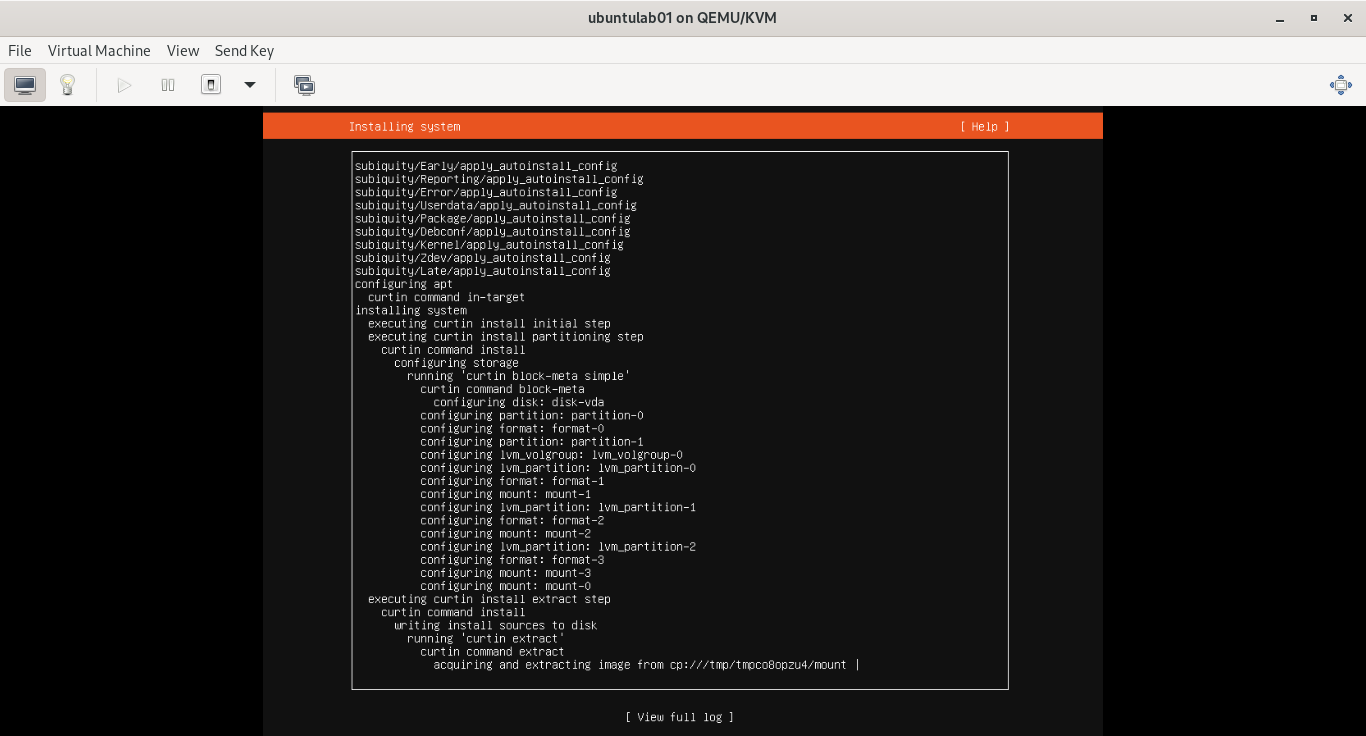
\includegraphics[scale=0.30]{16}
	\caption{Instalación del sistema base.}
\end{figure}

Prueba final del sistema, con su particionado correcto, recordemos que usamos BTRFS como sistema de ficheros bajo LVM.

\begin{figure}[H]
	\centering
	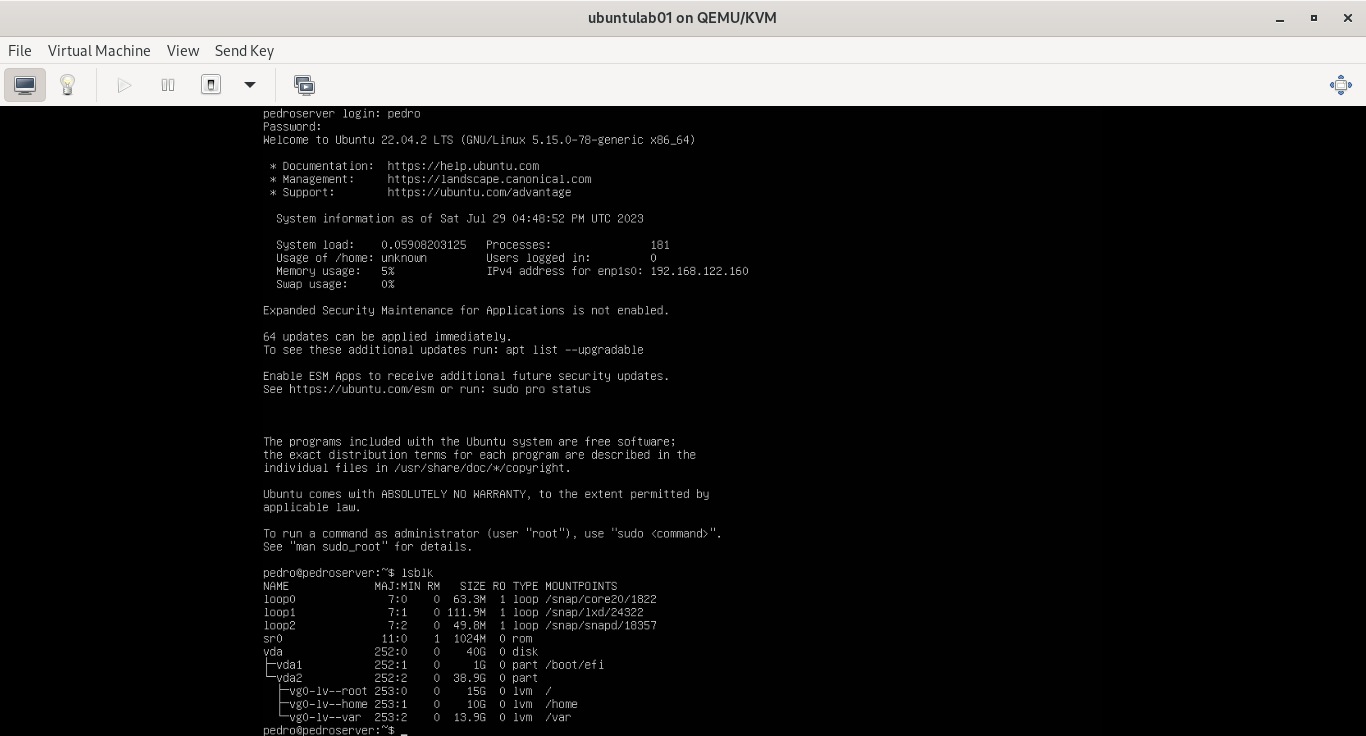
\includegraphics[scale=0.30]{17}
	\caption{lsblk como demostración.}
\end{figure}



% \vspace{5mm}


% \begin{lstlisting}[style=mybash]
%     # Para una base de datos concreta
%     mysqldump --user=tiendabd --password=password --databases tiendabd --add-drop-database --add-drop-table [--replace] --host=127.0.0.1 --result-file=dump.sql
% \end{lstlisting}



%\begin{figure}[H]
%	\centering
%	\includegraphics[scale=0.40]{cuestion_1_1}
%	\caption{Se puede ver que al no haber un fallo grave, el sistema lo nota como que sigue funcionando pero en un estado degradado.}
%\end{figure}

%\newpage

%Se pueden hacer include en latex
%\newpage

\section{Section}

\subsection{Subseccion}

\subsubsection{Subseccion}



%-------Bibliografia-----------------------------

%\newpage
\section{Bibliografía}

% Ejemplo
\footnote{Administración de mdadm - Por Red Hat}
\textcolor{blue}{\url{https://access.redhat.com/documentation/en-us/red_hat_enterprise_linux/8/html/managing_storage_devices/managing-raid_managing-storage-devices#monitoring-raid_managing-raid}}



\end{document}
